\subsection{Experimental Results}\label{subsec:experimental-results}

\subsubsection{Input Workpiece Variation}\label{subsubsec:input-workpiece-variation}

\subsubsection{Pause Duration Variation}\label{subsubsec:pause-duration-variation}

\begin{figure}
    \centering
    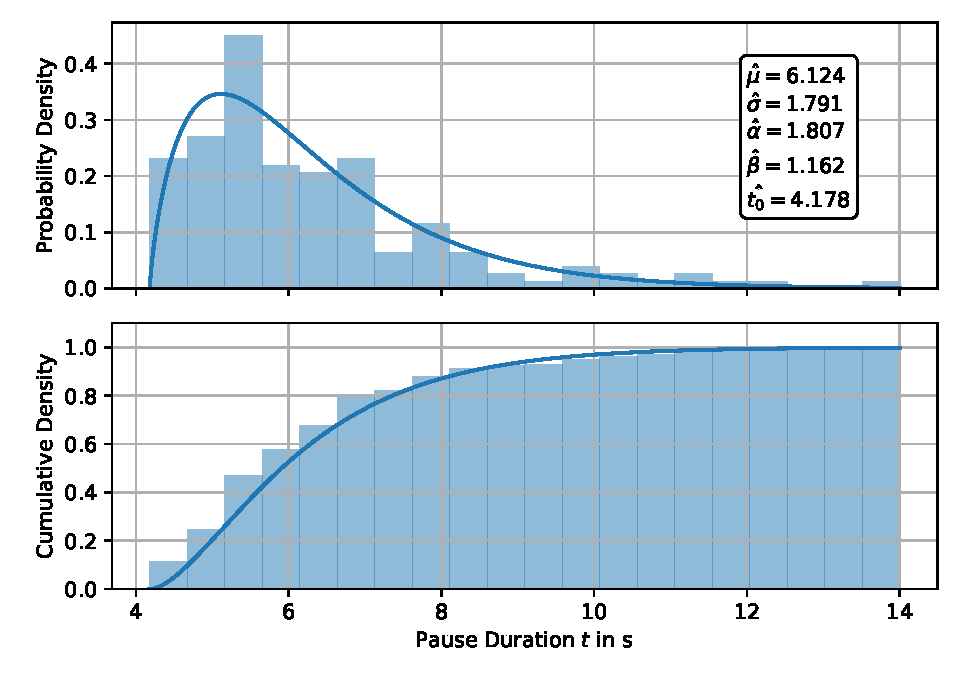
\includegraphics[width=\linewidth]{img/plot_histogram_pauses}
    \caption{Density and Cumulative Histograms of Inter-Pass Durations With Fitted Gamma Distribution}
    \label{fig:plot_histogram_pauses}
\end{figure}

\subsection{Simulation Results}\label{subsec:simulation-results}

In the following, three questions shall be investigated and answered:
\begin{enumerate}
    \item What is the difference in behavior of variations sourced in the input workpiece and arising within the process?
    \item What is the influence of elastic mill response on the variational behavior of the process?
    \item Is there a minimum number of passes needed to eliminate variations of the input workpiece?
\end{enumerate}

For this distinct simulations were carried out and compared with each other and the experimental data.

\subsubsection{Different Sources of Variation}\label{subsubsec:different-sources-of-variation}

Two basic classes of variation sources in can be identified in rolling processes, or manufacturing processes in general: variations inherent to the input workpiece and variations arising in the regarded processes itself.
These effect together the variation of the resulting product.
To investigate the different behavior of them, two simulations shall be carried out and compared.
The first one only regards variations of the input workpiece and how they evolve during the process.
The second one introduces additional variations within the process in means of varying inter-stand pause durations between the reversing passes.
These originate, as denoted before, in the manual handling of the workpiece for feeding into the next pass.
The focus of the following analysis lies on the temperature evolution of the workpiece, since this is crucial for microstructure evolution and final material properties, and will, presumably, be heavily effected by varying pause durations.

\begin{figure}
    \begin{subfigure}{\linewidth}
        \centering
        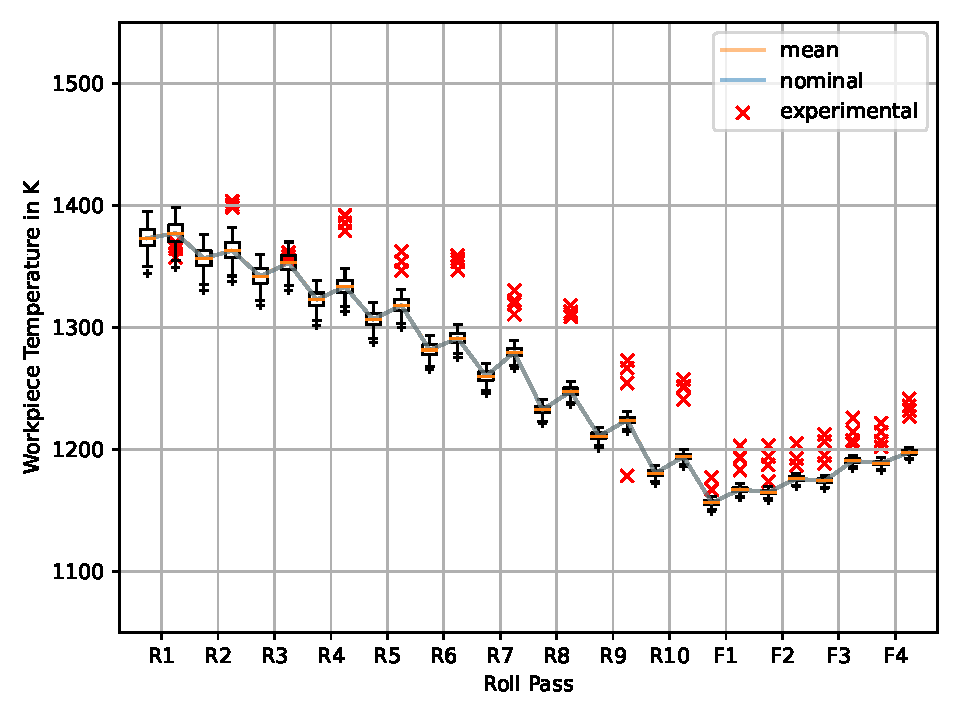
\includegraphics{img/input_temperature}
        \caption{Under Influence of Input Workpiece Variation}
        \label{fig:input_temperature}
    \end{subfigure}
    \begin{subfigure}{\linewidth}
        \centering
        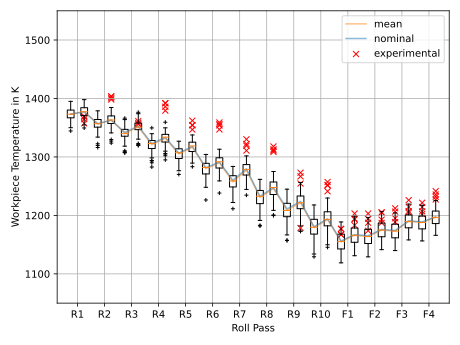
\includegraphics{img/durations_temperature}
        \caption{Under Influence of Input Workpiece Variation and Pause Duration Variation}
        \label{fig:durations_temperature}
    \end{subfigure}
    \caption{Variation of Workpiece Temperature}
\end{figure}


The temperature evolution of the first case is shown in \autoref{fig:input_temperature}.
The variation of the input workpiece was taken as obtained in \autoref{subsubsec:input-workpiece-variation}.
The box plots in the figure show the variation of the workpiece temperature, where the box marks a distance of $\Estimated\StandardDeviation$ to $\Estimated\Mean$ and the whiskers a distance of $3\Estimated\StandardDeviation$.
The variation of temperature decreases with each processing step and is remarkably small in the product.

The second case, however, is shown in \autoref{fig:durations_temperature}.
Here, the variation is not decreasing with each step, but increasing in the transport steps.
In contrast, roll passes still decrease the variation.
If the overall variation decreases in the process, depends, of course, on the ratio between decrease in passes and increase in transports.
In this view, the goal of process design must be to prevent an overall increase of variation in the process.
The main vantage point for this is to limit variation in pause durations.

\begin{figure}
    \centering
    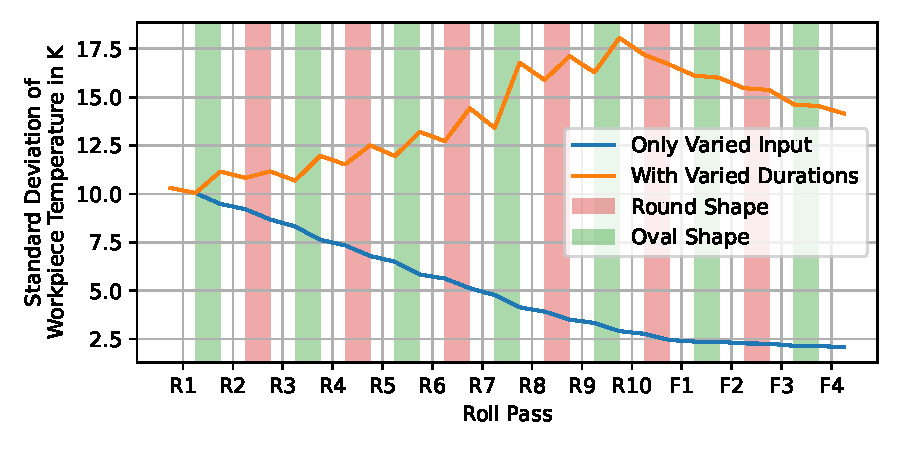
\includegraphics{img/temperature_std}
    \caption{Comparison of Temperature Variation Evolution Between Input Variation and Process Variation}
    \label{fig:temperature_std}
\end{figure}

\autoref{fig:temperature_std} shows the evolution of variation of both cases in comparison.
One can see, that the overall variation is increasing solely in the reversing transport for the second case.
Note, that the influence of transports in oval cross-section shape is remarkably higher than those in round shape.
This can be explained by the adverse surface area to volume ratio of oval cross-sections.

% Correlation Temperature Change <-> Variance Influence ?
% Stellschrauben: Temperaturverlust im Transport begrenzen, Temperaturanstieg im Walzstich erhöhen

% Vergleich Korngröße

\subsubsection{Influence of Elastic Mill Response}\label{subsubsec:influence-of-elastic-mill-response}

\subsubsection{Elimination of Input Variation}\label{subsubsec:elimination-of-input-variation}

